% Supplementary material as a stand-alone PDF (CVPR asks for it as a separate upload).
%
% How to build:
%   Overleaf : open this file (supp.tex) and click Recompile, then download the PDF.
%              If Overleaf still shows the full paper, set Menu -> Main document -> supp.tex,
%              recompile, and set it back to main.tex afterwards.
%   Locally  : pdflatex supp   (run it three times; no bibtex needed)
%
% The content lives in sec/X_suppl.tex, the same file that main.tex appends when it sets \suppltrue.
% Keep the three items marked KEEP IN SYNC identical to main.tex.

\documentclass[10pt,twocolumn,letterpaper]{article}

\usepackage[review]{cvpr}      % KEEP IN SYNC with main.tex (review / camera-ready)

% preamble.tex loads hyperref itself, so the link options are handed over before it is read.
% Giving them in a second \usepackage[...]{hyperref} afterwards is an "Option clash" error and
% leaves the links as boxes.
\definecolor{cvprblue}{rgb}{0.21,0.49,0.74}
\PassOptionsToPackage{pagebackref,breaklinks,colorlinks,allcolors=cvprblue}{hyperref}
%% Packages and layout tweaks, loaded by main.tex and rebuttal.tex before hyperref.
%%
%% Already loaded by cvpr.sty -- do NOT load again (option clashes):
%%   times, xspace, xcolor[dvipsnames], graphicx, amsmath, amssymb, booktabs,
%%   natbib, caption, subcaption, url, etoolbox, enumitem, cleveref (after hyperref)
%% Project macros (notes, method name, notation, table helpers) live in macros.tex.

%% ---------------------------------------------------------------------------
%% Packages
%% ---------------------------------------------------------------------------
\usepackage{multirow}    % \multirow in tables
\usepackage{tabularx}    % X columns that fill \linewidth
\usepackage{lipsum}
\usepackage{booktabs}
\usepackage{amsmath}
\usepackage{makecell}
\usepackage{array} 
\usepackage{colortbl}    % \rowcolor / \cellcolor (xcolor is already loaded)
\usepackage{bm}          % bold math symbols, \bm{x}
\usepackage{pifont}
\usepackage{amssymb}    
% \ding symbols for \cmark / \xmark
\usepackage{color}
\usepackage{colortbl}
\usepackage{subcaption}
% \renewcommand{\thesubtable}{(\alph{subtable})}
% \captionsetup[subtable]{labelformat=simple}

% Uncomment if needed:
% \usepackage{algorithm}
% \usepackage{algpseudocode}
% \usepackage{wrapfig}
% \usepackage{siunitx}   % aligned numeric columns, e.g. S[table-format=2.1]
\DeclareMathOperator*{\argtopk}{arg\,top-K}

% \newcommand{\red}[1]{{\color{red}#1}}
\newcommand{\orange}[1]{{\color{orange}#1}}
\newcommand{\blue}[1]{{\color{cyan}#1}}
\newcommand{\gray}[1]{{\color{gray}#1}}
%% ---------------------------------------------------------------------------
%% Paths
%% ---------------------------------------------------------------------------
\newcommand{\paragrapht}[1]{\noindent\textbf{#1}} 
\graphicspath{{figures/}}

% \newcommand{\cmark}{\ding{51}}%
% \newcommand{\xmark}{\ding{55}}%

\newcommand\blfootnote[1]{%
  \begingroup
  \renewcommand\thefootnote{}\footnote{#1}%
  \addtocounter{footnote}{-1}%
  \endgroup
}

\usepackage{xspace}
% \usepackage{multirow}
\usepackage{array}
\usepackage{layouts}
\usepackage{algorithm}
\usepackage{bbding}
\usepackage{listings}
\usepackage{pifont}
\usepackage{wasysym}
\usepackage{float}
\usepackage{soul}
\usepackage{footnote}
\makesavenoteenv{tabular}
\makesavenoteenv{table}
\makesavenoteenv{figure}
\usepackage{pythonhighlight}
\usepackage{enumitem}
\usepackage{graphicx}
\usepackage{wrapfig}
\usepackage{bbm}

\usepackage{hyperref}
\usepackage[capitalize,noabbrev]{cleveref}
\usepackage{tikz}
\usepackage{threeparttable}
\usetikzlibrary{patterns,patterns.meta}

\newcommand{\ji}[1]{\textcolor{blue}{#1}}
\newcommand{\cj}[1]{\textcolor{magenta}{#1}}

%% ---------------------------------------------------------------------------
%% Layout tweaks -- enable only near the end, when fighting the page limit
%% ---------------------------------------------------------------------------
% Tighter text layout (typically saves ~1/6 page):
% \usepackage{microtype}

% Compact run-in paragraph headings:
% \renewcommand{\paragraph}[1]{\vspace{.5em}\noindent\textbf{#1.}}

% Less space between figure and caption:
% \setlength{\abovecaptionskip}{.5em}

% Less space around floats:
% \setlength{\textfloatsep}{10pt plus 2pt minus 2pt}
% \setlength{\dbltextfloatsep}{10pt plus 2pt minus 2pt}

% Tighter underline:
% \usepackage{soul}
% \setuldepth{foobar}

% Supplement-only compatibility for the verbatim copy-repository draft.
% The original main-paper preamble above and its behavior are preserved.
\AtEndPreamble{%
  \ifdefined\supponly
    \usepackage[T1]{fontenc}
    \usepackage{placeins}
    \AtBeginDocument{%
    \crefname{figure}{figure}{figures}
    \Crefname{figure}{Figure}{Figures}
    \crefname{table}{table}{tables}
    \Crefname{table}{Table}{Tables}
    \crefname{section}{section}{sections}
    \Crefname{section}{Section}{Sections}
    \crefname{equation}{equation}{equations}
    \Crefname{equation}{Equation}{Equations}
    \crefname{algorithm}{algorithm}{algorithms}
    \Crefname{algorithm}{Algorithm}{Algorithms}
    }
  \fi
}

\usepackage{hyperref}

%% Project macros, loaded after hyperref by main.tex and rebuttal.tex.

%% ===========================================================================
%% Draft switch: set \draftfalse before submission -- every \TODO and \note
%% disappears and \todo / \red text turns black.
%% ===========================================================================
\newif\ifdraft
\drafttrue

\ifdraft
  \newcommand{\TODO}[1]{\textbf{\color{red}[TODO: #1]}}   % missing content
  \newcommand{\todo}[1]{{\color{red}#1}}                  % text that needs revision
  \newcommand{\red}[1]{{\color{red}#1}}
  \newcommand{\note}[2]{{\color{blue}[\textbf{#1}: #2]}}  % \note{YW}{comment}
\else
  \newcommand{\TODO}[1]{}
  \newcommand{\todo}[1]{#1}
  \newcommand{\red}[1]{#1}
  \newcommand{\note}[2]{}
\fi

%% ===========================================================================
%% Names (rename in one place)
%% ===========================================================================
\newcommand{\method}{ARROW\xspace}

%% ===========================================================================
%% Notation
%% ===========================================================================
\newcommand{\R}{\mathbb{R}}
\newcommand{\E}{\mathbb{E}}
\DeclareMathOperator*{\argmin}{arg\,min}
\DeclareMathOperator*{\argmax}{arg\,max}
\newcommand{\norm}[1]{\left\lVert#1\right\rVert}
\newcommand{\abs}[1]{\left\lvert#1\right\rvert}

%% ===========================================================================
%% Tables
%% ===========================================================================
\newcommand{\cmark}{\ding{51}}                              % check mark
\newcommand{\xmark}{\ding{55}}                              % cross
\newcommand{\best}[1]{\textbf{#1}}
\newcommand{\second}[1]{\underline{#1}}
\newcommand{\gain}[1]{{\scriptsize\color{ForestGreen}(+#1)}} % \gain{4.6}
\newcommand{\drop}[1]{{\scriptsize\color{BrickRed}(-#1)}}    % \drop{3.0}
\newcommand{\pp}{\,pp\xspace}                                % percentage points
\newcommand{\oursrow}{\rowcolor{cvprblue!8}}                 % shade "ours" rows

%% ===========================================================================
%% Figures: gray box with the final size, until the real figure exists.
%%   \placeholder{3cm}                 -> full column width, 3 cm tall
%%   \placeholder[0.48\linewidth]{3cm} -> custom width
%% ===========================================================================
\newcommand{\placeholder}[2][\linewidth]{%
  \fbox{\parbox[c][#2][c]{\dimexpr #1-2\fboxsep-2\fboxrule\relax}%
    {\centering\small\color{gray}placeholder}}}


\def\paperID{*****} % KEEP IN SYNC with main.tex
\def\confName{CVPR}
\def\confYear{2027}

\title{ARROW: Action-Aware Resolution Routing for World Action Models \\
-Supplementary Material-} % KEEP IN SYNC with main.tex

% Tells sec/X_suppl.tex that the main paper is not part of this PDF, so references to its
% tables are printed as fixed numbers ("Table 1 of the main paper") instead of cross-references.
\def\supponly{}

\begin{document}
\maketitle
\appendix

% Section-prefixed numbering (e.g., Eq. A.1, Table B.1, Fig. D.1) following PCME
\makeatletter
\renewcommand{\theequation}{\Alph{section}.\arabic{equation}}
\renewcommand{\thetable}{\Alph{section}.\arabic{table}}
\renewcommand{\thefigure}{\Alph{section}.\arabic{figure}}
\@addtoreset{equation}{section}
\@addtoreset{table}{section}
\@addtoreset{figure}{section}
\makeatother

\section*{Appendix}
    This document provides additional implementation details, quantitative analyses, and qualitative results to complement the main paper.
    \cref{app:exp_details} describes the mathematical formulation, benchmark protocols, token allocation schedules, baseline adaptations, and training hyperparameters.
    \cref{app:add_analysis} presents equal-token baseline comparisons, extended ablations, offline action-distortion curves, semantic region coverage, and per-task breakdowns.
    \cref{app:qual_analysis} provides spatial and temporal routing visualizations, real-robot rollout comparisons, and failure case analyses.

\section{Experimental Details}
\label{app:exp_details}

\subsection{Architecture and training formulation}
\label{app:supp_formulation}

\paragraph{Router architecture and gradient saliency.}
% Detail cross-attention head count, hidden dimension, MLP width, parameter/FLOPs overhead,
% the multiplicative straight-through estimator gate, and the derivation of Eq. (3).

\paragraph{Router objective and target smoothing.}
% Write explicit equations for L_focal, L_budget, and L_entropy in Eq. (4),
% along with the EMA decay rate used to smooth r_g and top-k (k = F) labeling.

\paragraph{Temporal boundary placement and positional indexing.}
% Formalize cumulative frame-to-frame cosine variation for placing K_p segment boundaries,
% native-grid spatial alignment, and 3D RoPE behavior under contiguous-t vs. source-t.

\paragraph{Velocity distillation and adapter merging.}
% Detail shared action-noise sampling in Eq. (2), linear folding of rank-16 LoRA weights
% at deployment, and training/inference pseudocode (Algorithms A.1--A.2).

\subsection{Benchmarks and evaluation protocols}
\label{app:supp_benchmarks}

\paragraph{LIBERO.}
% Detail LIBERO-Spatial, LIBERO-Object, and LIBERO-Goal (10 tasks each, 50 episodes,
% 3 paired seeds, 5-step execution horizon, and exclusion of LIBERO-Long).

\paragraph{SIMPLER-Bridge.}
% Detail the 4 WidowX tasks, 96 paired evaluation episodes, observation/action horizons,
% and released mimic-video checkpoint configuration.

\paragraph{RoboCasa-GR1.}
% Detail the 24 tabletop manipulation tasks, 1,200 paired evaluation episodes,
% observation inputs, and DiT4DiT checkpoint configuration.

\paragraph{Real-robot kitchen tasks.}
% Detail the 7-DoF Franka Emika Panda arm, Robotiq-2F-85 gripper, side-view 480x640 RGB camera,
% exact task definitions and success criteria for all 6 tasks in Fig. 6 / Tab. 5, and 15 trials per task.

\subsection{Allocation schedules and hyperparameters}
\label{app:supp_schedules}

\paragraph{Token budgets and tier schedules.}
% Include Table A.1: observation/future token counts, routing block index, spatial full-res groups F,
% and priority-tier segment counts K_p for mimic-video and DiT4DiT across all benchmarks.

\paragraph{Optimization hyperparameters.}
% Include Table A.2 (modeled on BLIP-2 Tables 7--9): optimizer, learning rate, schedule,
% batch size, training steps, LoRA rank/alpha/targets, and loss weights.

\paragraph{Inference profiling and statistical testing.}
% Detail H100 and RTX 4090 batch-1 latency/FLOPs measurement protocols, paired 95% CIs,
% and Holm-corrected paired McNemar significance tests (including the degree symbol in Tab. 4).

\subsection{Baseline adaptation protocols}
\label{app:supp_baselines}

\paragraph{FastV-style.}
% Detail shallow block-2 visual self-attention ranking, matched-budget pruning,
% and dedicated rank-16 decoder LoRA training.

\paragraph{VLA-Pruner.}
% Detail semantic instruction attention combined with historical action-decoder attention,
% dense bootstrap queries per episode, and mean token accounting (*) in Tab. 1.

\paragraph{ADP.}
% Detail text-guided token selection, end-effector motion-gate thresholds triggering
% full-context fallback queries, and mean token accounting (*) in Tab. 1.

\paragraph{CF-Prune.}
% Detail the two-pass single-step adaptation: initial full-context probe pass for instruction
% and action attention followed by pruned prediction, and its latency/FLOPs accounting.
\section{Additional Analysis}
\label{app:add_analysis}

\subsection{Equal-token baseline comparisons}
\label{app:supp_equal_token}

\paragraph{Fixed-budget evaluation on mimic-video.}
% Include Table B.1: strict equal-token comparison on LIBERO with dense bootstrap and
% motion-gated fallback queries disabled for VLA-Pruner and ADP at 4,080 / 5,760 / 7,440 tokens.

\paragraph{Fixed-budget evaluation on DiT4DiT.}
% Include Table B.2: strict equal-token comparison on LIBERO at 391 / 442 / 589 tokens,
% isolating single-pass selector accuracy from dense fallback calls.

\subsection{Extended ablation studies}
\label{app:supp_ablations}

\paragraph{Routing layer depth.}
% Include Table B.3a: varying the shallow DiT block index where ARROW is applied,
% analyzing the trade-off between feature maturity and latency reduction.

\paragraph{Router and distillation objectives.}
% Include Table B.3b: ablating L_focal, L_budget, L_entropy, STE gradient supervision,
% and velocity distillation vs. ground-truth-only LoRA supervision (\lambda_GT).

\paragraph{Spatial and temporal budget allocation.}
% Include Table B.3c: comparing spatial-only, temporal-only, and joint two-stage allocation,
% as well as varying full-resolution group count F under a fixed budget N.

\paragraph{Temporal priority and segment boundaries.}
% Include Table B.3d: comparing u_p = S_{g(p)} * \Delta_p against relevance-only or
% dynamics-only scoring, and equal-variation vs. uniform segment pooling.

\subsection{Offline distortion and coverage analysis}
\label{app:supp_diagnostics}

\paragraph{Task-agnostic and oracle scoring criteria.}
% Define the five task-agnostic criteria (similarity, motion, block-2 self-attention,
% edge energy, random) and the full-context decoder-attention oracle from Sec. 4.3.

\paragraph{Insertion and ranking-reversal curves.}
% Include Figure B.1 (promised in Sec. 4.3): offline spatial coarsening insertion curves
% and ranking-reversal plots corresponding to the distortion ratios (0.495--0.838).

\paragraph{Semantic region coverage across suites.}
% Include Figure B.2 (promised in Sec. 4.3) and Table B.4: simulator pixel coverage on
% LIBERO-Object and LIBERO-Goal, plus region-wise selection breakdown on LIBERO and Bridge.

\subsection{Per-task results and statistical tests}
\label{app:supp_pertask}

\paragraph{Per-task breakdown on simulation benchmarks.}
% Include Tables B.5--B.6: task-by-task success rates across LIBERO (30 tasks),
% SIMPLER-Bridge (4 tasks), and RoboCasa-GR1 (24 tasks).

\paragraph{Detailed statistical significance results.}
% Include Table B.7: paired differences, 95% CIs, and Holm-corrected paired McNemar p-values
% for main comparisons (Tab. 1) and operator/adaptation ablations (Tabs. 3--4).
\FloatBarrier
\section{Qualitative Analysis}
\label{app:qual_analysis}


\subsection{Spatiotemporal routing visualizations}
\label{app:supp_vis_routing}

\newcommand{\selimg}[2]{\includegraphics[width=0.188\textwidth]{supp/sel_#1_#2.pdf}}
\begin{figure*}[!t]
  \centering
  \setlength{\tabcolsep}{1.5pt}
  \renewcommand{\arraystretch}{1.0}
  \begin{tabular}{@{}c@{\hspace{3pt}}ccccc@{}}
    & \footnotesize FastV-style & \footnotesize VLA-Pruner & \footnotesize ADP & \footnotesize CF-Prune & \footnotesize\textbf{\method} \\[1pt]
    \rotatebox[origin=c]{90}{\footnotesize LIBERO-Spatial} &
    \raisebox{-0.5\height}{\selimg{libero}{fastv}} & \raisebox{-0.5\height}{\selimg{libero}{vlapruner}} &
    \raisebox{-0.5\height}{\selimg{libero}{adp}} & \raisebox{-0.5\height}{\selimg{libero}{cfprune}} &
    \raisebox{-0.5\height}{\selimg{libero}{arrow}} \\[2pt]
    \rotatebox[origin=c]{90}{\footnotesize LIBERO-Goal} &
    \raisebox{-0.5\height}{\selimg{goal}{fastv}} & \raisebox{-0.5\height}{\selimg{goal}{vlapruner}} &
    \raisebox{-0.5\height}{\selimg{goal}{adp}} & \raisebox{-0.5\height}{\selimg{goal}{cfprune}} &
    \raisebox{-0.5\height}{\selimg{goal}{arrow}} \\[2pt]
    \rotatebox[origin=c]{90}{\footnotesize LIBERO-Object} &
    \raisebox{-0.5\height}{\selimg{object}{fastv}} & \raisebox{-0.5\height}{\selimg{object}{vlapruner}} &
    \raisebox{-0.5\height}{\selimg{object}{adp}} & \raisebox{-0.5\height}{\selimg{object}{cfprune}} &
    \raisebox{-0.5\height}{\selimg{object}{arrow}} \\[2pt]
    \rotatebox[origin=c]{90}{\footnotesize SIMPLER-Bridge} &
    \raisebox{-0.5\height}{\selimg{bridge}{fastv}} & \raisebox{-0.5\height}{\selimg{bridge}{vlapruner}} &
    \raisebox{-0.5\height}{\selimg{bridge}{adp}} & \raisebox{-0.5\height}{\selimg{bridge}{cfprune}} &
    \raisebox{-0.5\height}{\selimg{bridge}{arrow}} \\[2pt]
    \rotatebox[origin=c]{90}{\footnotesize RoboCasa-GR1} &
    \raisebox{-0.5\height}{\selimg{robocasa}{fastv}} & \raisebox{-0.5\height}{\selimg{robocasa}{vlapruner}} &
    \raisebox{-0.5\height}{\selimg{robocasa}{adp}} & \raisebox{-0.5\height}{\selimg{robocasa}{cfprune}} &
    \raisebox{-0.5\height}{\selimg{robocasa}{arrow}} \\
  \end{tabular}
  \caption{\textbf{Spatial group selection of five rules on the same frame.}
  Within a row, every rule keeps the same number of $2{\times}2$ groups of the same observation; for the baselines this is their selection component at a fixed budget, not their deployed policy.
  \raisebox{0.15ex}{
\includegraphics[height=0.9ex]{supp/legend_region.pdf}}/\raisebox{0.15ex}{
\includegraphics[height=0.9ex]{supp/legend_arrow_region.pdf}}: selected groups (baselines/\method);
  \raisebox{0.15ex}{
\includegraphics[height=0.9ex]{supp/legend_object.pdf}}: task objects;
  \raisebox{0.15ex}{
\includegraphics[height=0.9ex]{supp/legend_path.pdf}}: future path of the end effector.
  LIBERO outlines and path come from simulator segmentation; 
  RoboCasa-GR1 (DiT4DiT) shows a demonstration frame with $7{\times}7$ groups, of which every rule keeps 16;  the black bars are letterbox padding. \cref{tab:supp_region_coverage} gives the averages over 50 episodes.}
  \label{fig:supp_selection_maps}
\end{figure*}



\paragraph{Spatial group selection across tasks.}

\suppdraft{\Cref{fig:supp_selection_maps}} shows the groups that each rule keeps from the same frame.
On LIBERO, FastV-style spends much of its budget on the table and the dark cabinet and misses the bowl to be picked up, ADP keeps the arm and the cabinet but misses the plate and most of the path, and VLA-Pruner's selection is scattered over the scene.
\suppdraft{In the illustrated LIBERO-Spatial frame, CF-Prune and \method both keep compact regions around the arm and task objects, while \method also retains groups along the future path between them. CF-Prune obtains its selection after a full-context probe.}
On Bridge, the baselines again select scattered regions or regions away from the target, while \method keeps the object, the path and the target pot, plus a few isolated groups along the top edge.

\suppdraft{The following pixel shares are single-frame measurements from \suppdraft{\cref{fig:supp_selection_maps}}. In its LIBERO-Goal frame, VLA-Pruner, CF-Prune and \method keep the arm, bowl and plate (\method covers 90\% of the plate), and \method keeps 43\% of the other-object pixels, compared with 49\% and 59\% for VLA-Pruner and CF-Prune. FastV-style misses both task objects and ADP misses the bowl.}
\suppdraft{In the single LIBERO-Object frame of \suppdraft{\cref{fig:supp_selection_maps}}, CF-Prune and VLA-Pruner keep nearly all of the sauce and basket, together with 99\% and 90\% of the other-object pixels. \method keeps 84\% of the basket, 70\% of the sauce and the path between them, with 20\% of the other-object pixels. FastV-style keeps the basket but not the sauce, and ADP keeps neither task object.}
\suppdraft{Across the 50-episode recordings in \suppdraft{\cref{tab:supp_region_coverage}}, \method has the highest mean future-path coverage among the five selection rules on each LIBERO suite: 82.3\% on Spatial, 77.0\% on Goal and 96.7\% on Object. These episode-averaged values describe the multi-episode analysis, separately from the single-frame pixel shares above.}

On RoboCasa-GR1, \method keeps the both pepper and the target basket in this frame.

\begin{figure*}[!t]
  \centering
  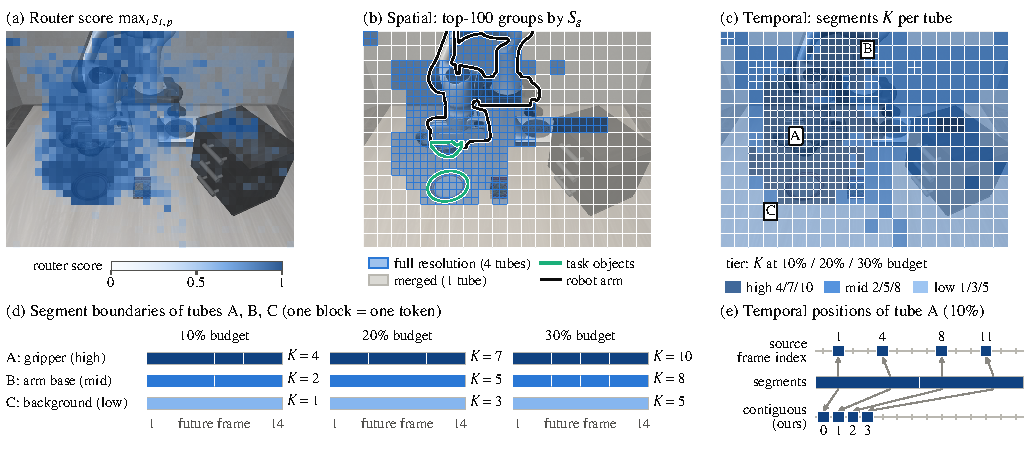
\includegraphics[width=\linewidth]{supp/allocation_steps.pdf}
  \caption{\textbf{Allocation of one recorded query, step by step.}
  LIBERO-Spatial, first task, recorded during a closed-loop rollout.
  (a) Router score $\max_t s_{t,p}$.
  (b) The 100 groups with the highest $S_g$ keep full resolution (four tubes); the others are merged into one tube.
  (c) Priority tier of every tube and its segment count $K$ at the 10/20/30\% budgets.
  (d) Segment boundaries of three tubes, one per tier; each block is one token.
  (e) Temporal positions of tube A at 10\%: source frames (source-t) versus consecutive indices (contiguous-t).}
  \label{fig:supp_allocation_steps}
\end{figure*}

\paragraph{Temporal tubelet segmentation.}

\suppdraft{\Cref{fig:supp_allocation_steps}} follows one recorded query through the allocation.
Tube A, on the gripper, is in the highest tier and receives 4, 7 and 10 segments at the three budgets; tube C, on the table background, is in the lowest tier and receives 1, 3 and 5.
Tube B, on the arm base, is in the middle tier because its router score is lower than the gripper's, not because its features change less.
Within each tube, the boundaries follow the cumulative feature change (\suppdraft{\cref{eq:supp_cuts}}), so segments are shorter where the features change faster, and contiguous-t gives the segments consecutive temporal positions (e).

\subsection{Real-robot rollout comparisons}
\label{app:supp_vis_robot}

\suppdraft{\Cref{fig:supp_real_robot_rollouts} shows recorded Full-context and \method rollouts on Stack Bowls and Open Lid, together with \method router scores aligned to the saved camera observations. The columns compare task phases in separate runs. The supplementary video provides additional real-robot demonstrations.}

\begin{figure*}[!t]
  \centering
  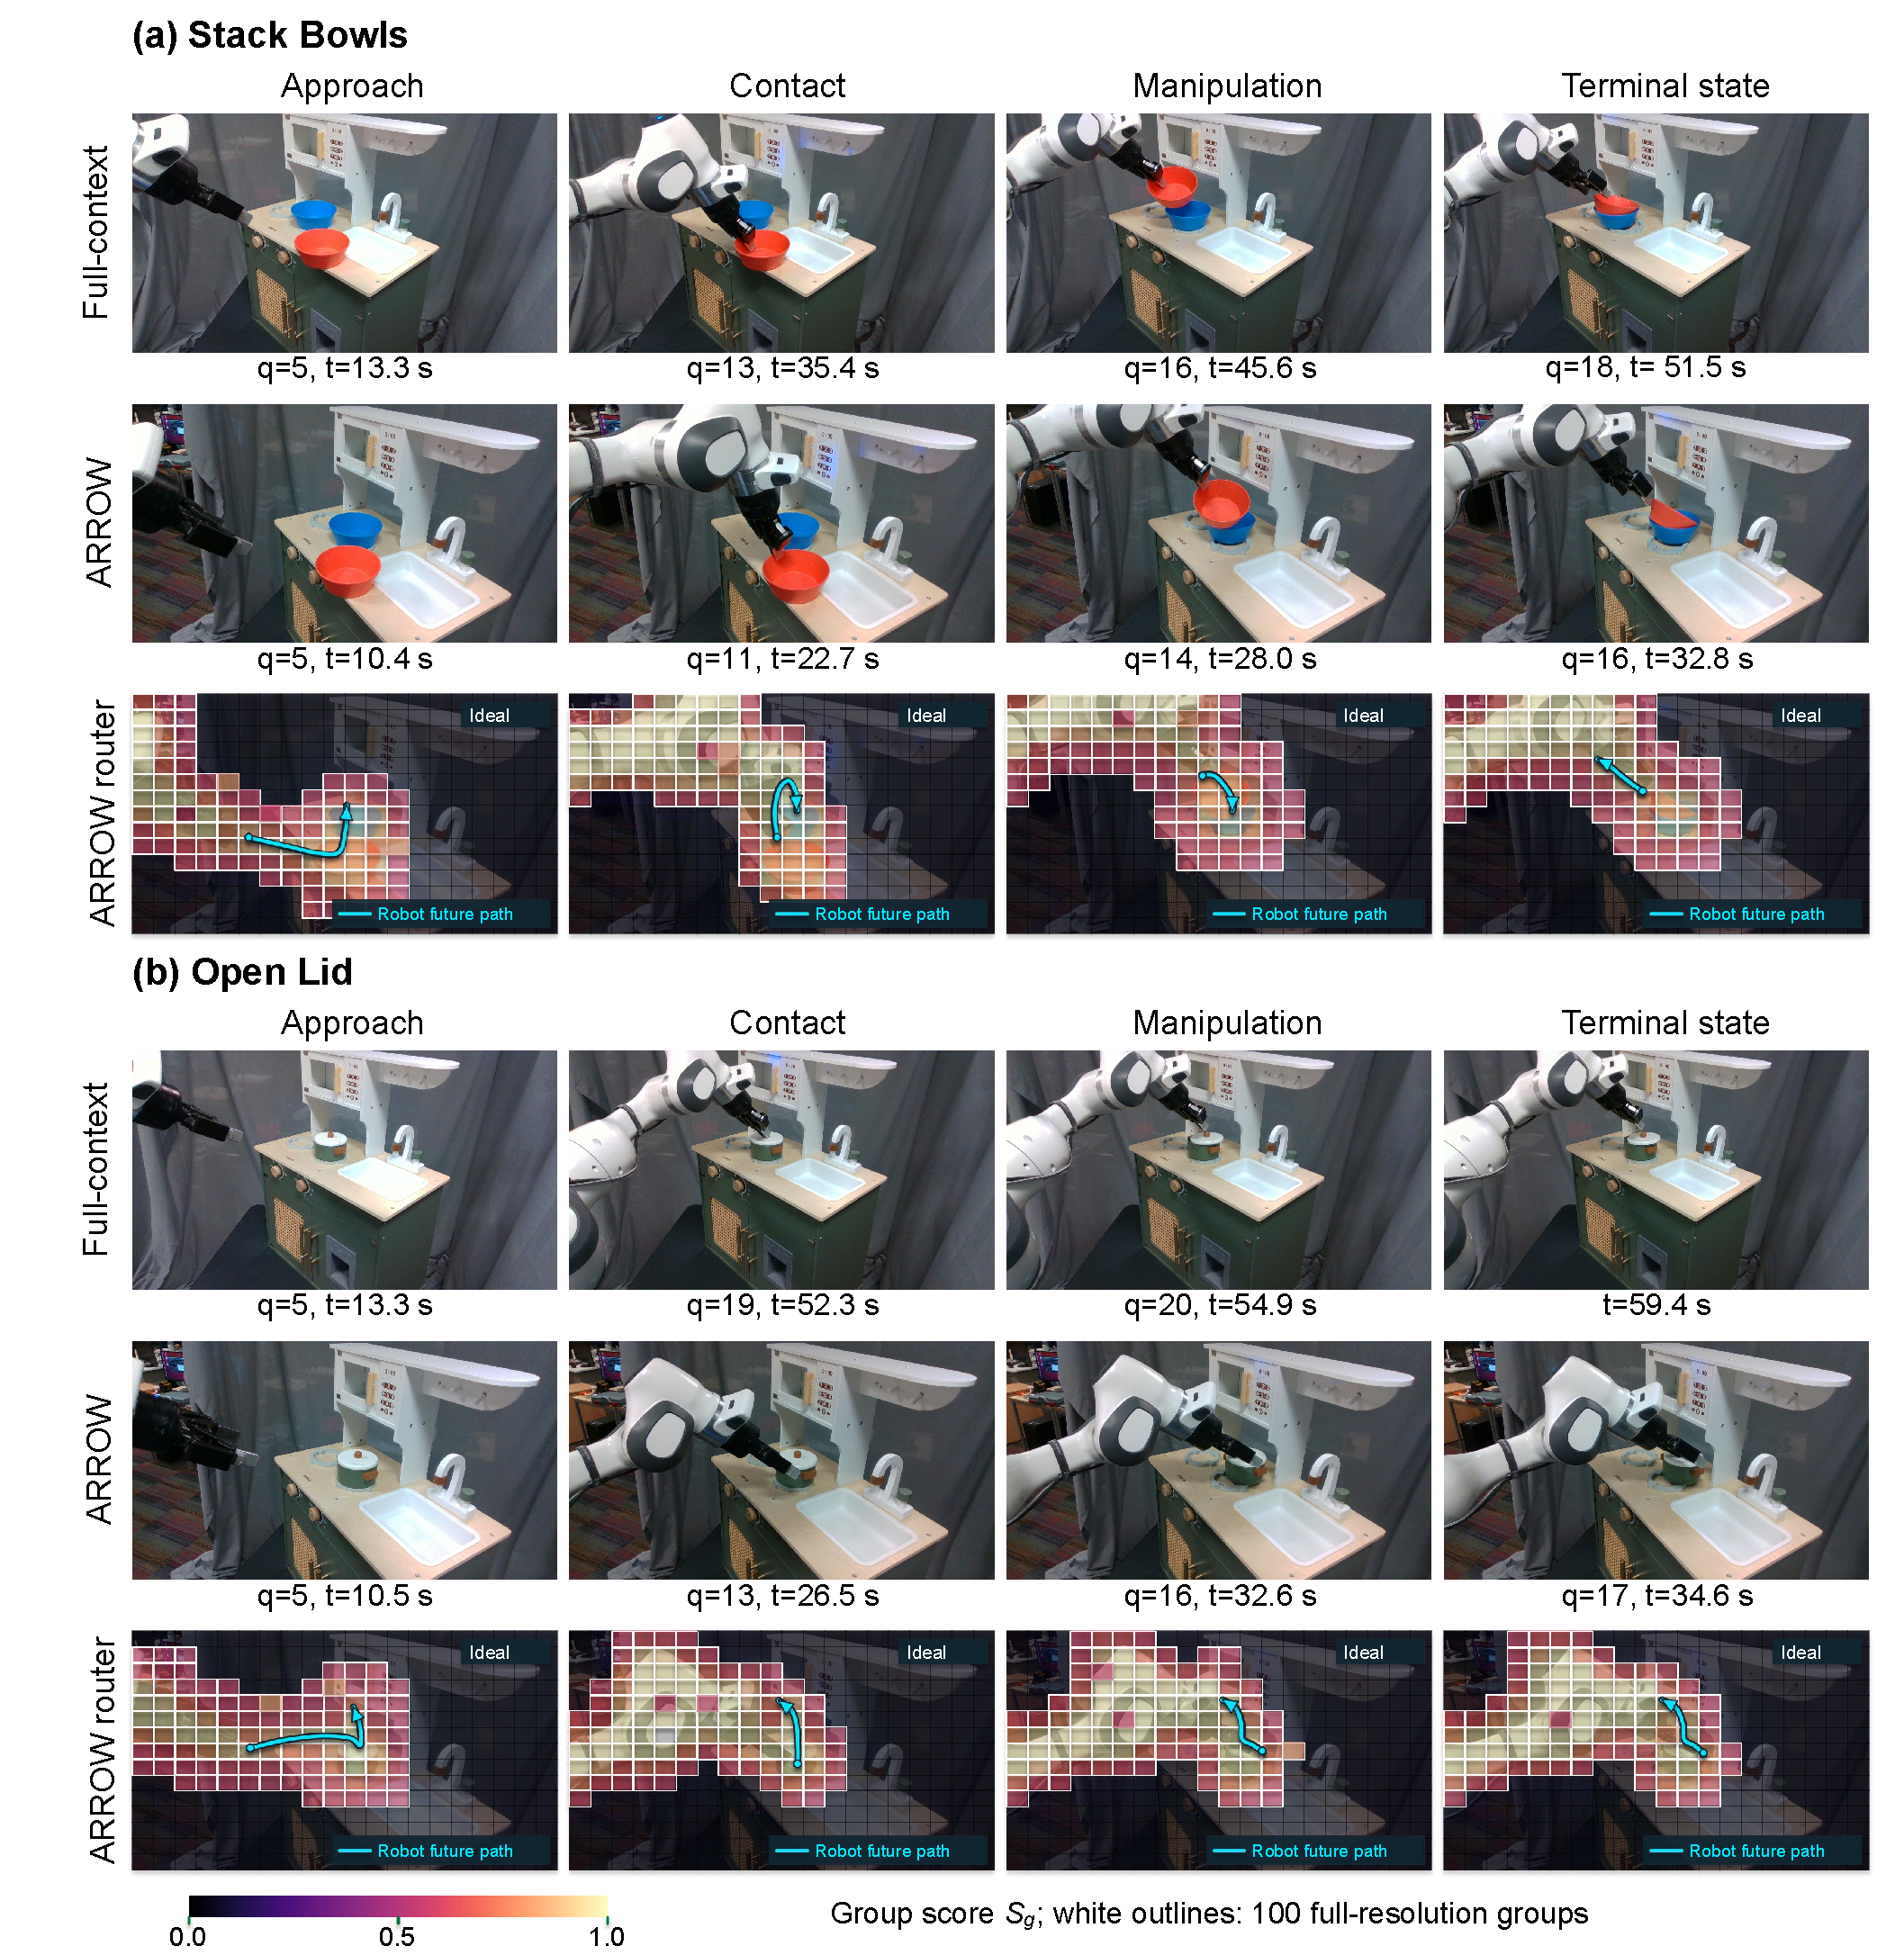
\includegraphics[width=\textwidth]{supp_real_robot_rollouts.pdf}
  \captionsetup{labelfont={color=suppdraftgreen}}
  \caption{\suppdraft{\textbf{Real-robot rollouts and camera-aligned routing.}
  (a) Stack Bowls; (b) Open Lid. Each task shows Full-context (19,200 tokens), \method (7,440 tokens, retaining 30\% of future tokens), and \method group scores $S_g$ over the corresponding observation.
  White outlines mark the 100 groups kept at full spatial resolution; all heatmaps use the same $[0,1]$ scale.
  Routing is reconstructed offline from the saved observation histories with the matching checkpoints; the replayed actions exactly match the recorded actions.
  Columns align separate rollouts by task phase, with query index $q$ and elapsed video time $t$.}}
  \label{fig:supp_real_robot_rollouts}
\end{figure*}

\subsection{Failure case analysis}
\label{app:supp_failures}


To avoid choosing failures by eye, we recorded 100 LIBERO-Spatial episodes of the 10\% policy (10 trials per task), with the frames, the simulator segmentation and the allocation of every query, and fixed the selection rule before the run.
Because trial $t$ of a task uses the same initial state in every run, each episode pairs with the full-context episode of the same task and trial.
    % \ji{Across the 100 LIBERO-Spatial episodes at the 10\% future token budget, over-compression primarily harms episodes where a small or partially occluded target object is coarsened into merged groups while distractor receptacles elsewhere on the table retain distinguish the commanded target }

\paragraph{Over-compression in cluttered scenes.}

\begin{figure*}[!t]
  \centering
  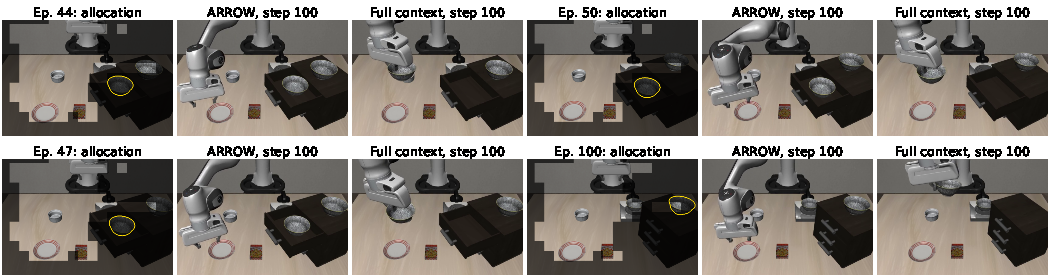
\includegraphics[width=\textwidth]{supp_failure_compression.pdf}
  \captionsetup{labelfont={color=suppdraftgreen}}
  \caption{\textbf{Failures observed at the 10\% budget.}
  Episodes that fail with \method and succeed with the full-context policy, ranked by the share of task-object pixels in merged groups over the last five queries before failure.
  Per episode, from left to right: the allocation at the first query (merged groups darkened, target bowl outlined), then the frame at step 100 of the 10\% policy and of the full-context policy from the same initial state.
  Episodes 44, 50 and 47 (bowl in the top drawer) have the highest shares (52, 51 and 49\%); episode 100 (bowl on the wooden cabinet) is the median of the 29 episodes (36\%).}
  \label{fig:supp_failure_compression}
\end{figure*}
\Cref{fig:supp_failure_compression} shows episodes that fail with \method but succeed with the full-context policy, ranked by the share of task-object pixels in merged groups during the last five queries before the failure is decided; we show the three highest and the median.
At 10\%, these failures concentrate on three Spatial tasks (\cref{tab:supp_pertask_libero}): picking the bowl from the top drawer, next to the cookie box, and from the wooden cabinet.

In all four shown episodes the arm never approaches the target bowl: it moves to the ramekin and the plate on the left of the table and stays there until the time limit, whereas the full-context policy, from the same initial state, lifts the bowl from the drawer or the cabinet top within 100 steps.
Throughout these episodes the allocation keeps the ramekin and the plate at full resolution, but none of the target bowl in the three drawer episodes and 27\% of it in the fourth.
The videos do not show why the arm goes to the ramekin; we note only that the ramekin stands where the bowl is picked up in two other tasks of the suite.

\paragraph{Failures shared with the base policy.}

\begin{figure*}[!t]
  \centering
  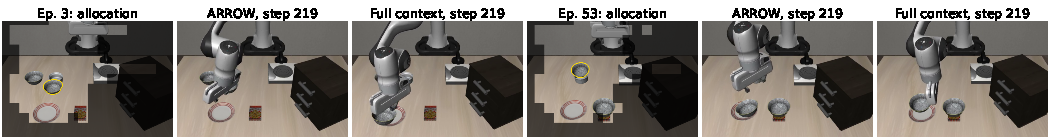
\includegraphics[width=\textwidth]{supp_failure_shared.pdf}
  \captionsetup{labelfont={color=suppdraftgreen}}
  \caption{\textbf{Failures shared with the full-context policy.}
  Episodes that fail with both policies although at least 90\% of the task-object and robot pixels are in full-resolution groups.
  Layout as in \cref{fig:supp_failure_compression}, at the last step (219); the target bowl is entirely at full resolution in both episodes.}
  \label{fig:supp_failure_shared}
\end{figure*}
\Cref{fig:supp_failure_shared} shows episodes that fail with both \method and the full-context policy although at least 90\% of the task-object and robot pixels are in full-resolution groups, ranked in the same way.
The allocation keeps most target-object and robot pixels at full resolution, but shared failure alone does not identify a common cause or exclude temporal compression and decoder adaptation.
Of the four episodes that fail with both policies, two meet this criterion.
In episode 3 (bowl between the plate and the ramekin), the 10\% policy closes the gripper above the bowl without lifting it and moves to the plate empty; the full-context policy lifts the bowl but still holds it at the plate when the time limit is reached.
In episode 53 (bowl on the ramekin), both policies carry the bowl to the plate and release it at the plate's edge, where it rests on the rim.
Only episode 53 therefore fails in the same way under both policies.

\end{document}
